\documentclass[tikz,border=12pt]{standalone}
\usepackage{graphicx}
\usepackage{amsmath,amssymb}
\usepackage{tikz}
\usetikzlibrary{arrows.meta,positioning,fit,calc,backgrounds}
\tikzset{
  box/.style={
    draw,
    very thick,
    rectangle,
    align=center,
    inner sep=8pt,
    minimum height=1.25cm,
    minimum width=3.1cm,
    font=\small,
  },
  wide/.style={box, minimum width=3.6cm},
  arr/.style={-{Stealth[length=2.6mm, width=2mm]}, thick},
  barr/.style={
    {Stealth[length=2.4mm, width=1.8mm]}-{Stealth[length=2.4mm, width=1.8mm]},
    thick,
  },
  lbl/.style={font=\scriptsize, inner sep=2pt, fill=white},
  group/.style={draw, dashed, inner sep=12pt},
}

\begin{document}
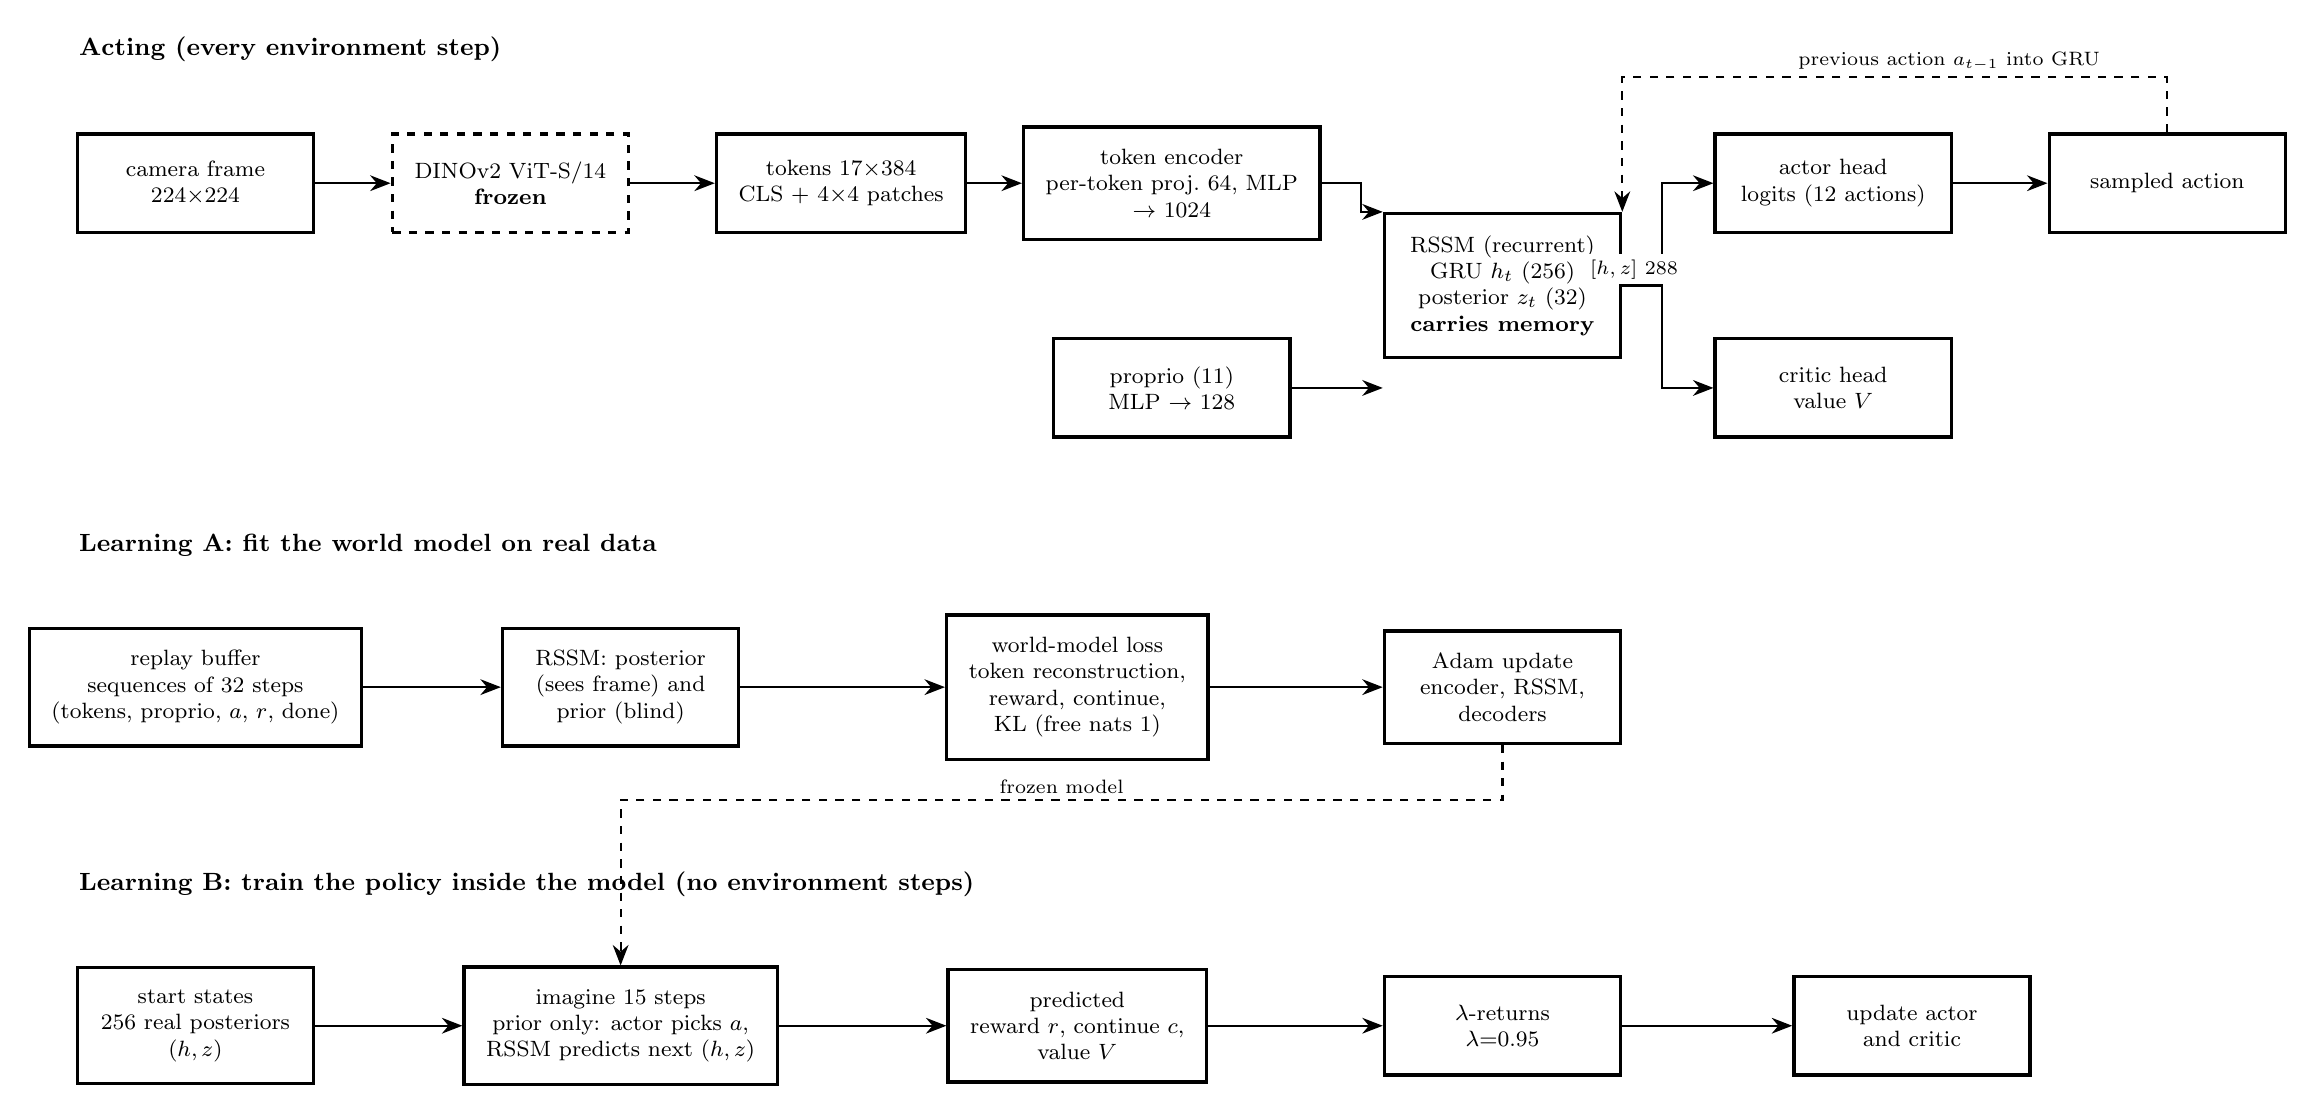
\begin{tikzpicture}
  \tikzset{box/.append style={minimum width=3.0cm, font=\footnotesize}}
  % ---------- acting ----------
  \node[font=\small\bfseries, anchor=west] at (-1.6,1.7) {Acting (every environment step)};
  \node[box] (frame) at (0,0) {camera frame\\$224{\times}224$};
  \node[box, dashed] (dino) at (4.0,0) {DINOv2 ViT-S/14\\\textbf{frozen}};
  \node[box] (tok) at (8.2,0) {tokens $17{\times}384$\\CLS $+$ $4{\times}4$ patches};
  \node[box] (enc) at (12.4,0) {token encoder\\per-token proj.\ 64, MLP\\$\to$ 1024};
  \node[box] (prop) at (12.4,-2.6) {proprio (11)\\MLP $\to$ 128};
  \node[box] (rssm) at (16.6,-1.3) {RSSM (recurrent)\\GRU $h_t$ (256)\\posterior $z_t$ (32)\\\textbf{carries memory}};
  \node[box] (act) at (20.8,0) {actor head\\logits (12 actions)};
  \node[box] (crit) at (20.8,-2.6) {critic head\\value $V$};
  \draw[arr] (frame) -- (dino);
  \draw[arr] (dino) -- (tok);
  \draw[arr] (tok) -- (enc);
  \draw[arr] (enc.east) -- ++(0.5,0) |- (rssm.north west |- rssm.north);
  \draw[arr] (prop.east) -- (rssm.west |- prop.east);
  \draw[arr] (rssm.east) -- node[lbl, above, pos=0.3] {$[h,z]$ 288} ++(0.5,0) |- (act.west);
  \draw[arr] (rssm.east) -- ++(0.5,0) |- (crit.west);
  \node[box, right=1.2cm of act] (a) {sampled action};
  \draw[arr] (act) -- (a);
  \draw[arr, dashed] (a.north) -- ++(0,0.7) -| node[lbl, above, pos=0.2] {previous action $a_{t-1}$ into GRU} (rssm.north east);

  % ---------- learning A: world model ----------
  \node[font=\small\bfseries, anchor=west] at (-1.6,-4.6) {Learning A: fit the world model on real data};
  \node[box] (rep) at (0,-6.4) {replay buffer\\sequences of 32 steps\\(tokens, proprio, $a$, $r$, done)};
  \node[box] (wm) at (5.4,-6.4) {RSSM: posterior\\(sees frame) and\\prior (blind)};
  \node[box] (wl) at (11.2,-6.4) {world-model loss\\token reconstruction,\\reward, continue,\\KL (free nats 1)};
  \node[box] (wu) at (16.6,-6.4) {Adam update\\encoder, RSSM,\\decoders};
  \draw[arr] (rep) -- (wm);
  \draw[arr] (wm) -- (wl);
  \draw[arr] (wl) -- (wu);

  % ---------- learning B: imagination ----------
  \node[font=\small\bfseries, anchor=west] at (-1.6,-8.9) {Learning B: train the policy inside the model (no environment steps)};
  \node[box] (st) at (0,-10.7) {start states\\256 real posteriors\\$(h,z)$};
  \node[box] (im) at (5.4,-10.7) {imagine 15 steps\\prior only: actor picks $a$,\\RSSM predicts next $(h,z)$};
  \node[box] (hr) at (11.2,-10.7) {predicted\\reward $r$, continue $c$,\\value $V$};
  \node[box] (lr) at (16.6,-10.7) {$\lambda$-returns\\$\lambda{=}0.95$};
  \node[box] (au) at (21.8,-10.7) {update actor\\and critic};
  \draw[arr] (st) -- (im);
  \draw[arr] (im) -- (hr);
  \draw[arr] (hr) -- (lr);
  \draw[arr] (lr) -- (au);
  \draw[arr, dashed] (wu.south) -- ++(0,-0.7) -| node[lbl, above, pos=0.25] {frozen model} (im.north);
\end{tikzpicture}
\end{document}
